\documentclass{article}

\usepackage[a4paper, margin=20mm]{geometry}
\usepackage{amsmath}
\usepackage{amsthm}
\usepackage{amssymb}
\usepackage{graphicx}
\usepackage{enumitem}


\def\c#1{\texttt{#1}}

\title{Homework 1 - Information Security (ICS344)}
\author{Alfaifi, Ammar}
\date{}

\begin{document}

\maketitle

\section{Installing VMs}
In my case I installed two virtual machines. The first one is pre-built \c{vbox} of \c{Kali Linux} distro.
The second VM, I chose install \c{Arch} Linux for its customiztion cababilities. The host operatin system is
\c{MacBook Pro (13-inch, 2016, Two Thunderbolt 3 ports)} with \c{VirtualBox} as my VM manager.

\section{Network Configuration}
See Figure~\ref{fig:net-change} for how I managed to change the netowrk settings for each VM.

\begin{figure}[ht]
	\centering
	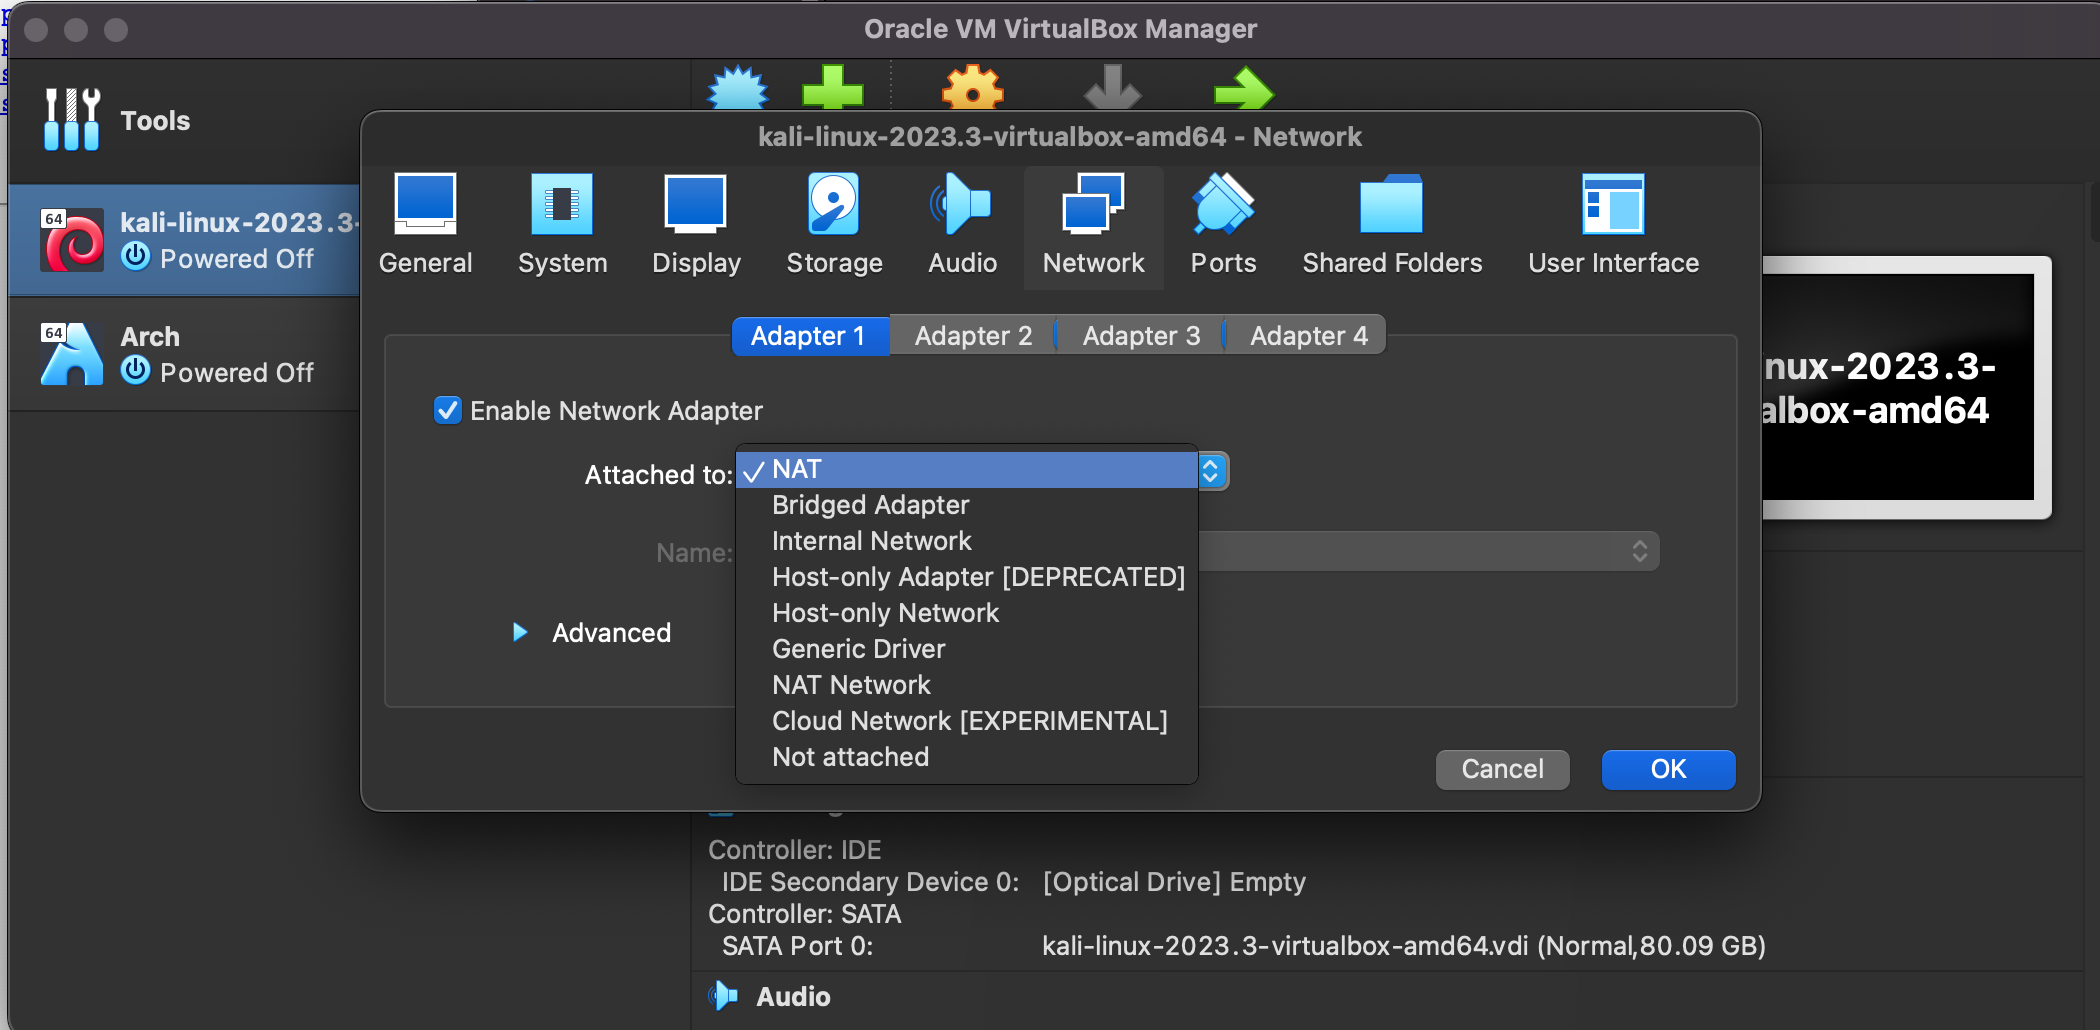
\includegraphics[width=0.6\textwidth]{figures/setting-network.png}
	\caption{Changing each VM's networking mode.}
	\label{fig:net-change}
\end{figure}

\subsection{Network Address Translation (NAT)}
NAT networking allows the virtual machine to share the host's IP address and network connection. The host acts as a router, and the virtual machine is assigned an IP address in a private, isolated network. The host performs Network Address Translation, translating traffic between the VM and the external network. See Figure~\ref{fig:nat-set} for the VMs' IP addresses.

\begin{figure}[ht]
	\begin{center}
		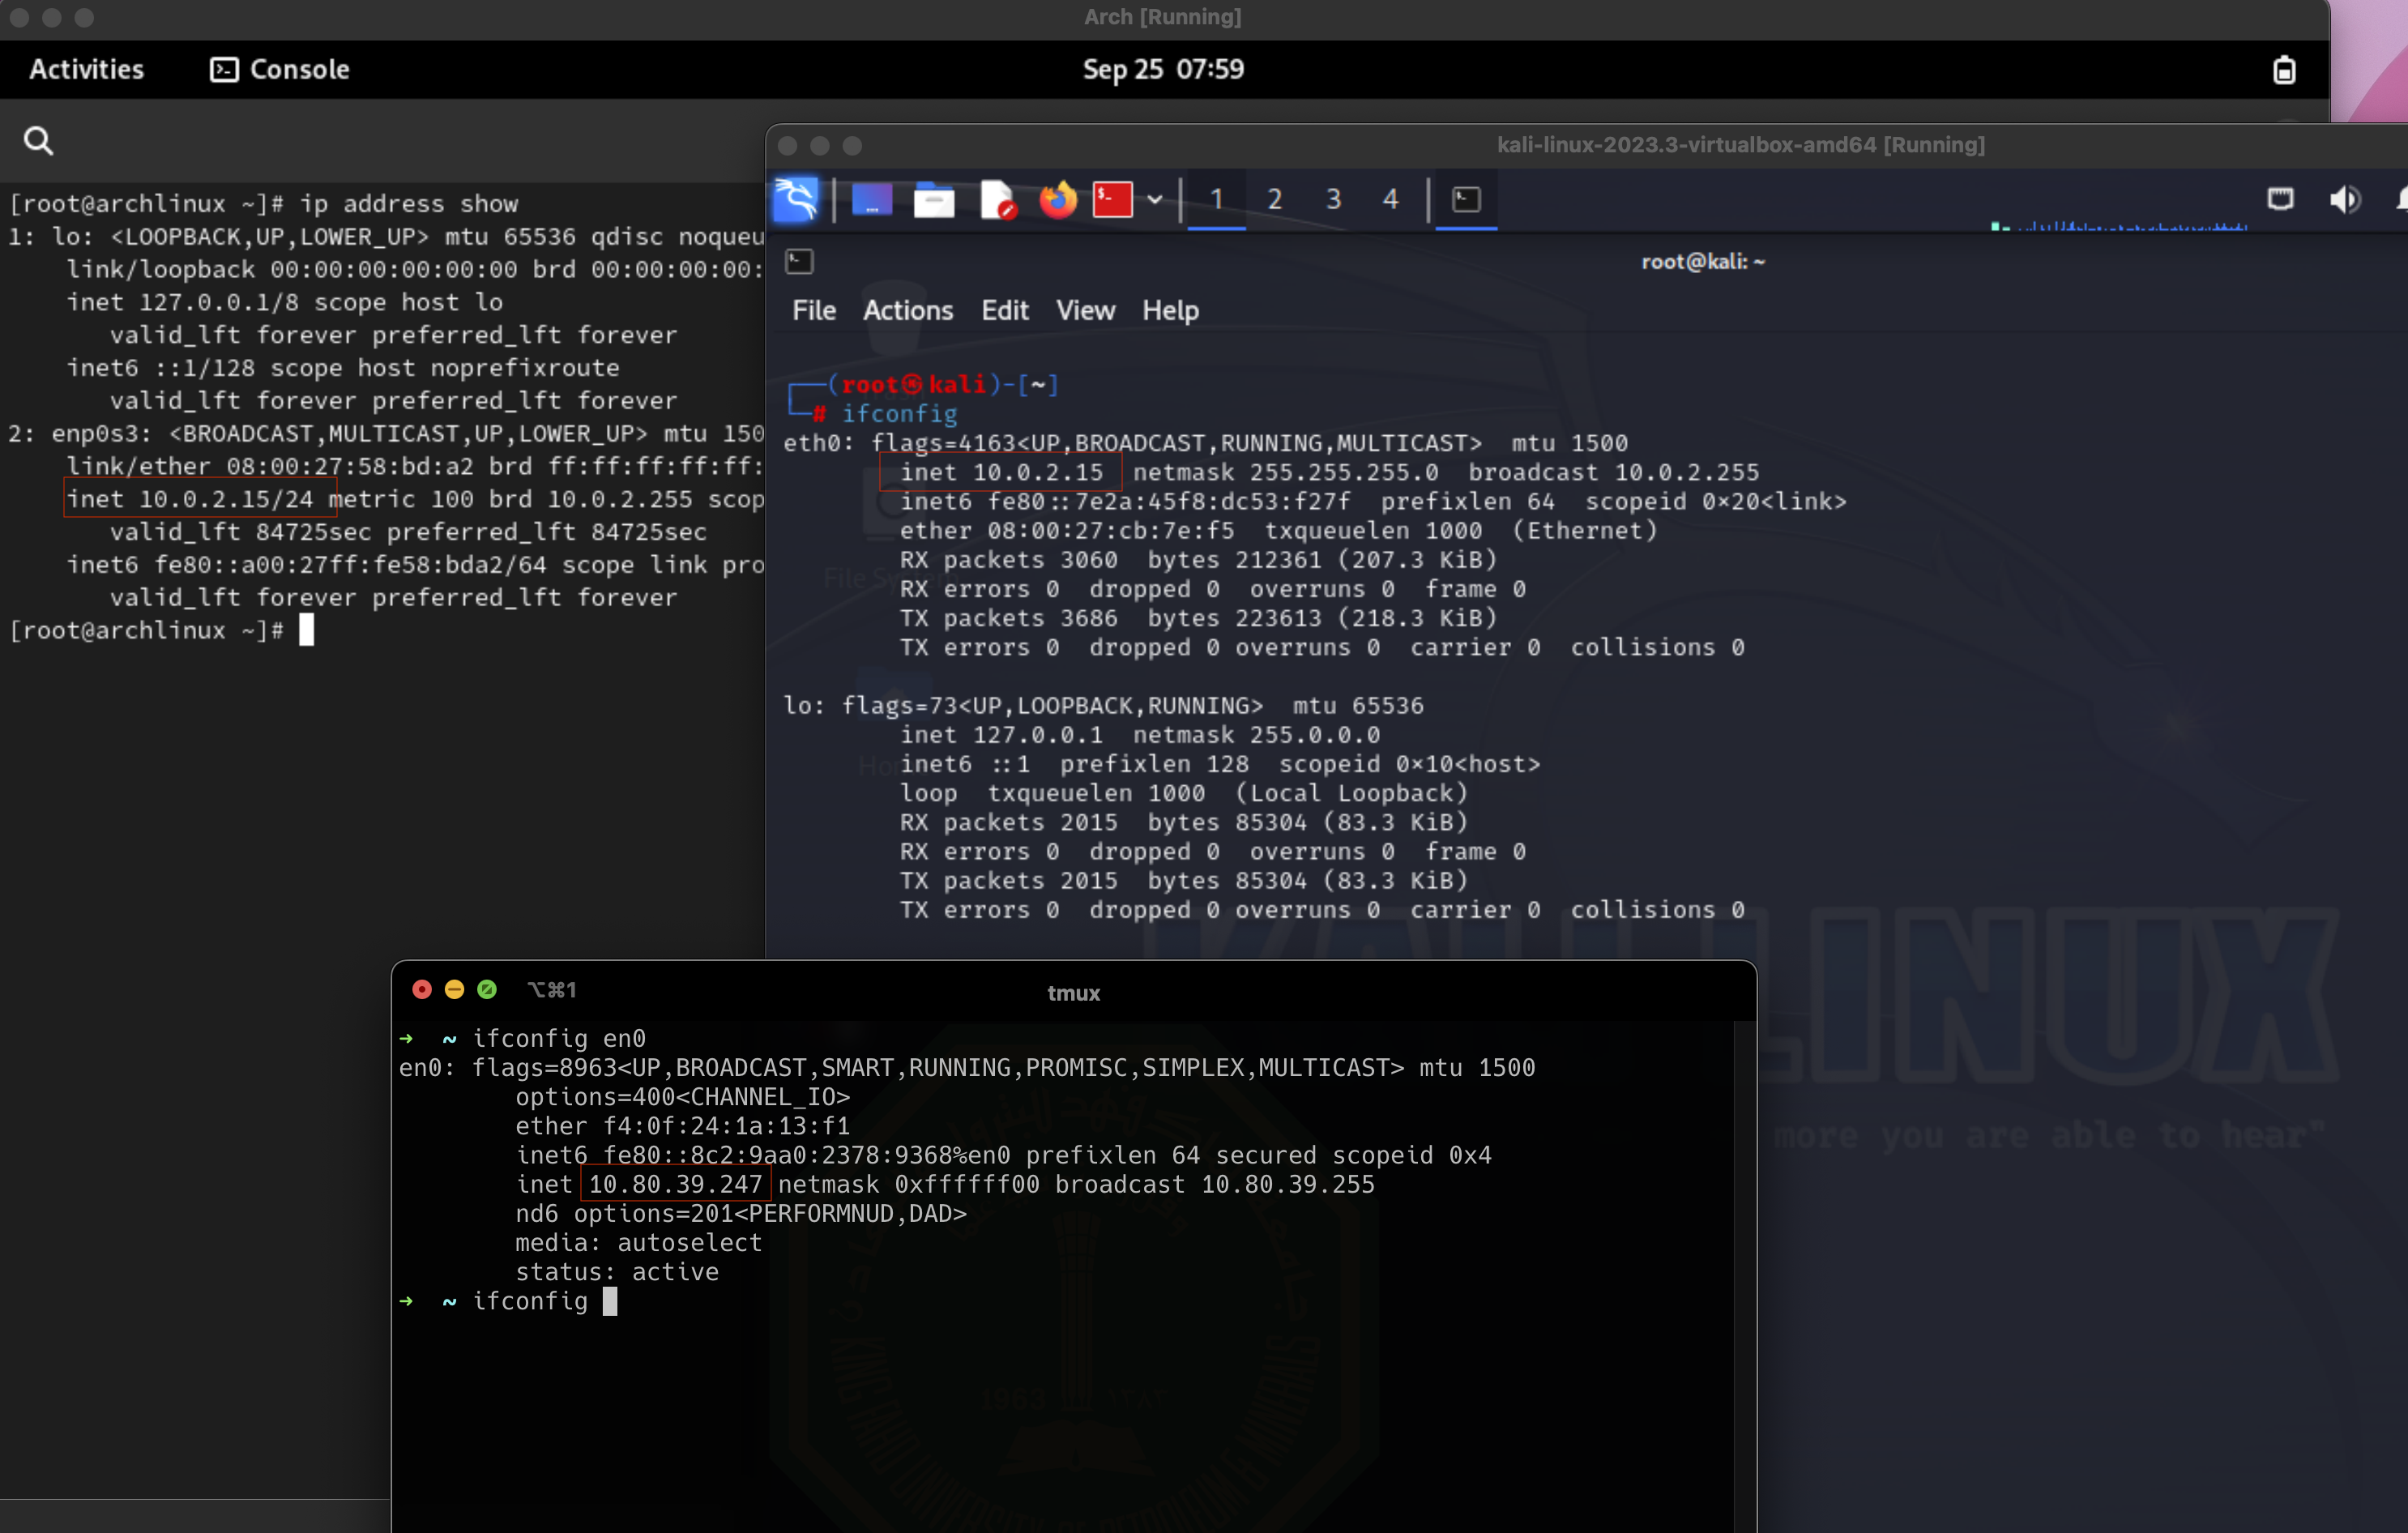
\includegraphics[width=0.95\textwidth]{figures/NAT-set.png}
	\end{center}
	\caption{Left window is Arch VM, the right window is Kali VM, and the middle window is terminal from the host OS. You can see the two VMs share the same IP address, while the hosting machine has its unique IP address.}
	\label{fig:nat-set}
\end{figure}

\subsection{Bridged Networking}
Bridged networking allows a virtual machine to appear as a separate device on the physical network to which your host computer is connected. This setting essentially bridges the virtual machine's network adapter with the host's network adapter, making it appear as if the virtual machine is directly connected to the physical network. See Figure~\ref{fig:bridge-section}; it appears that each VM it has its own IP address. As in Figure~\ref{fig:net-change} we change to `Bridge adapter', and in each VM's OS we set up the IP address and the gateway, as in Figure~\ref{fig:bridge-kali}.

\begin{figure}[ht]
	\begin{center}
		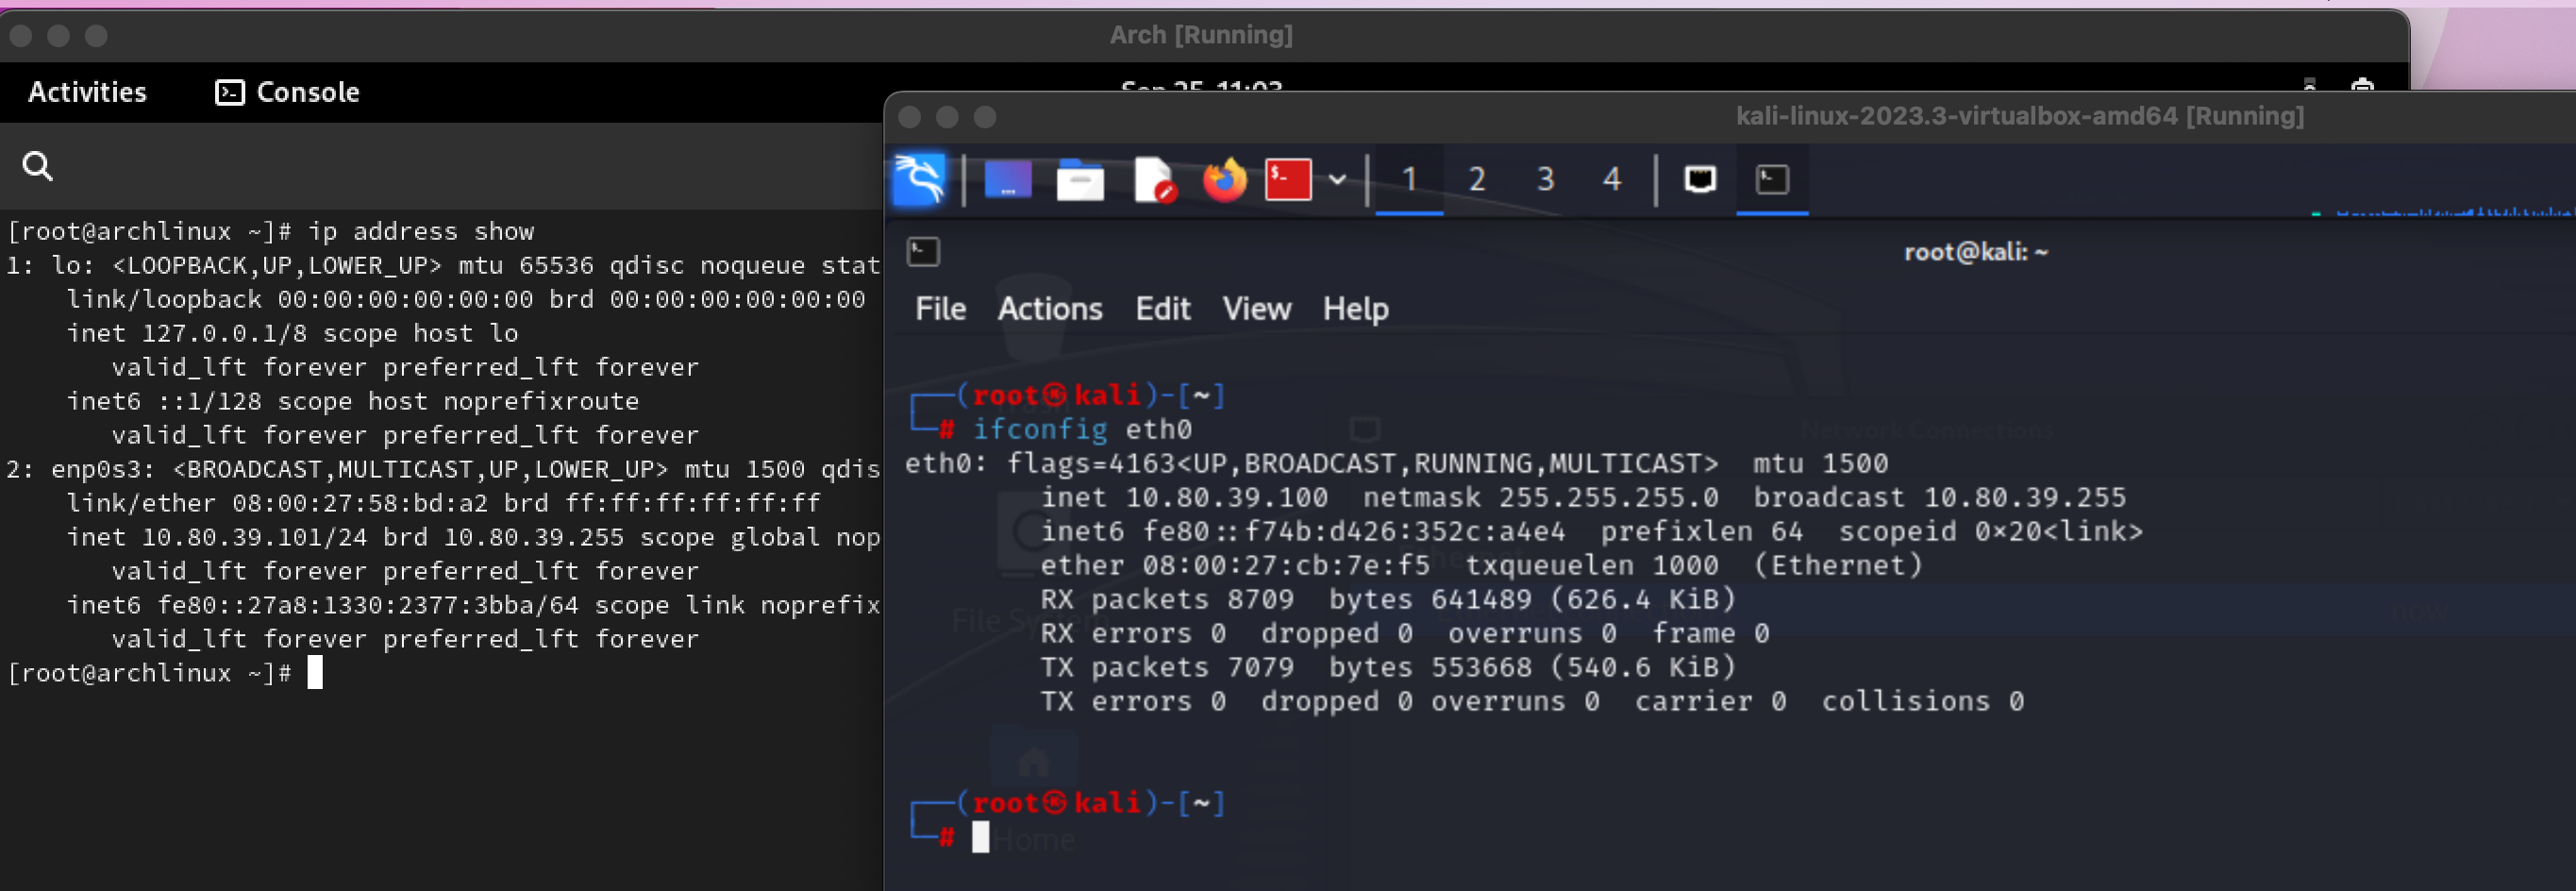
\includegraphics[width=0.95\textwidth]{figures/bridge-set.png}
	\end{center}
	\caption{We see that for each machine it has its own unique IP address withing \c{10.80.93.0/24} network. As if it was directly connected to the hosting machine network.}
	\label{fig:bridge-section}
\end{figure}

\begin{figure}
	\begin{center}
		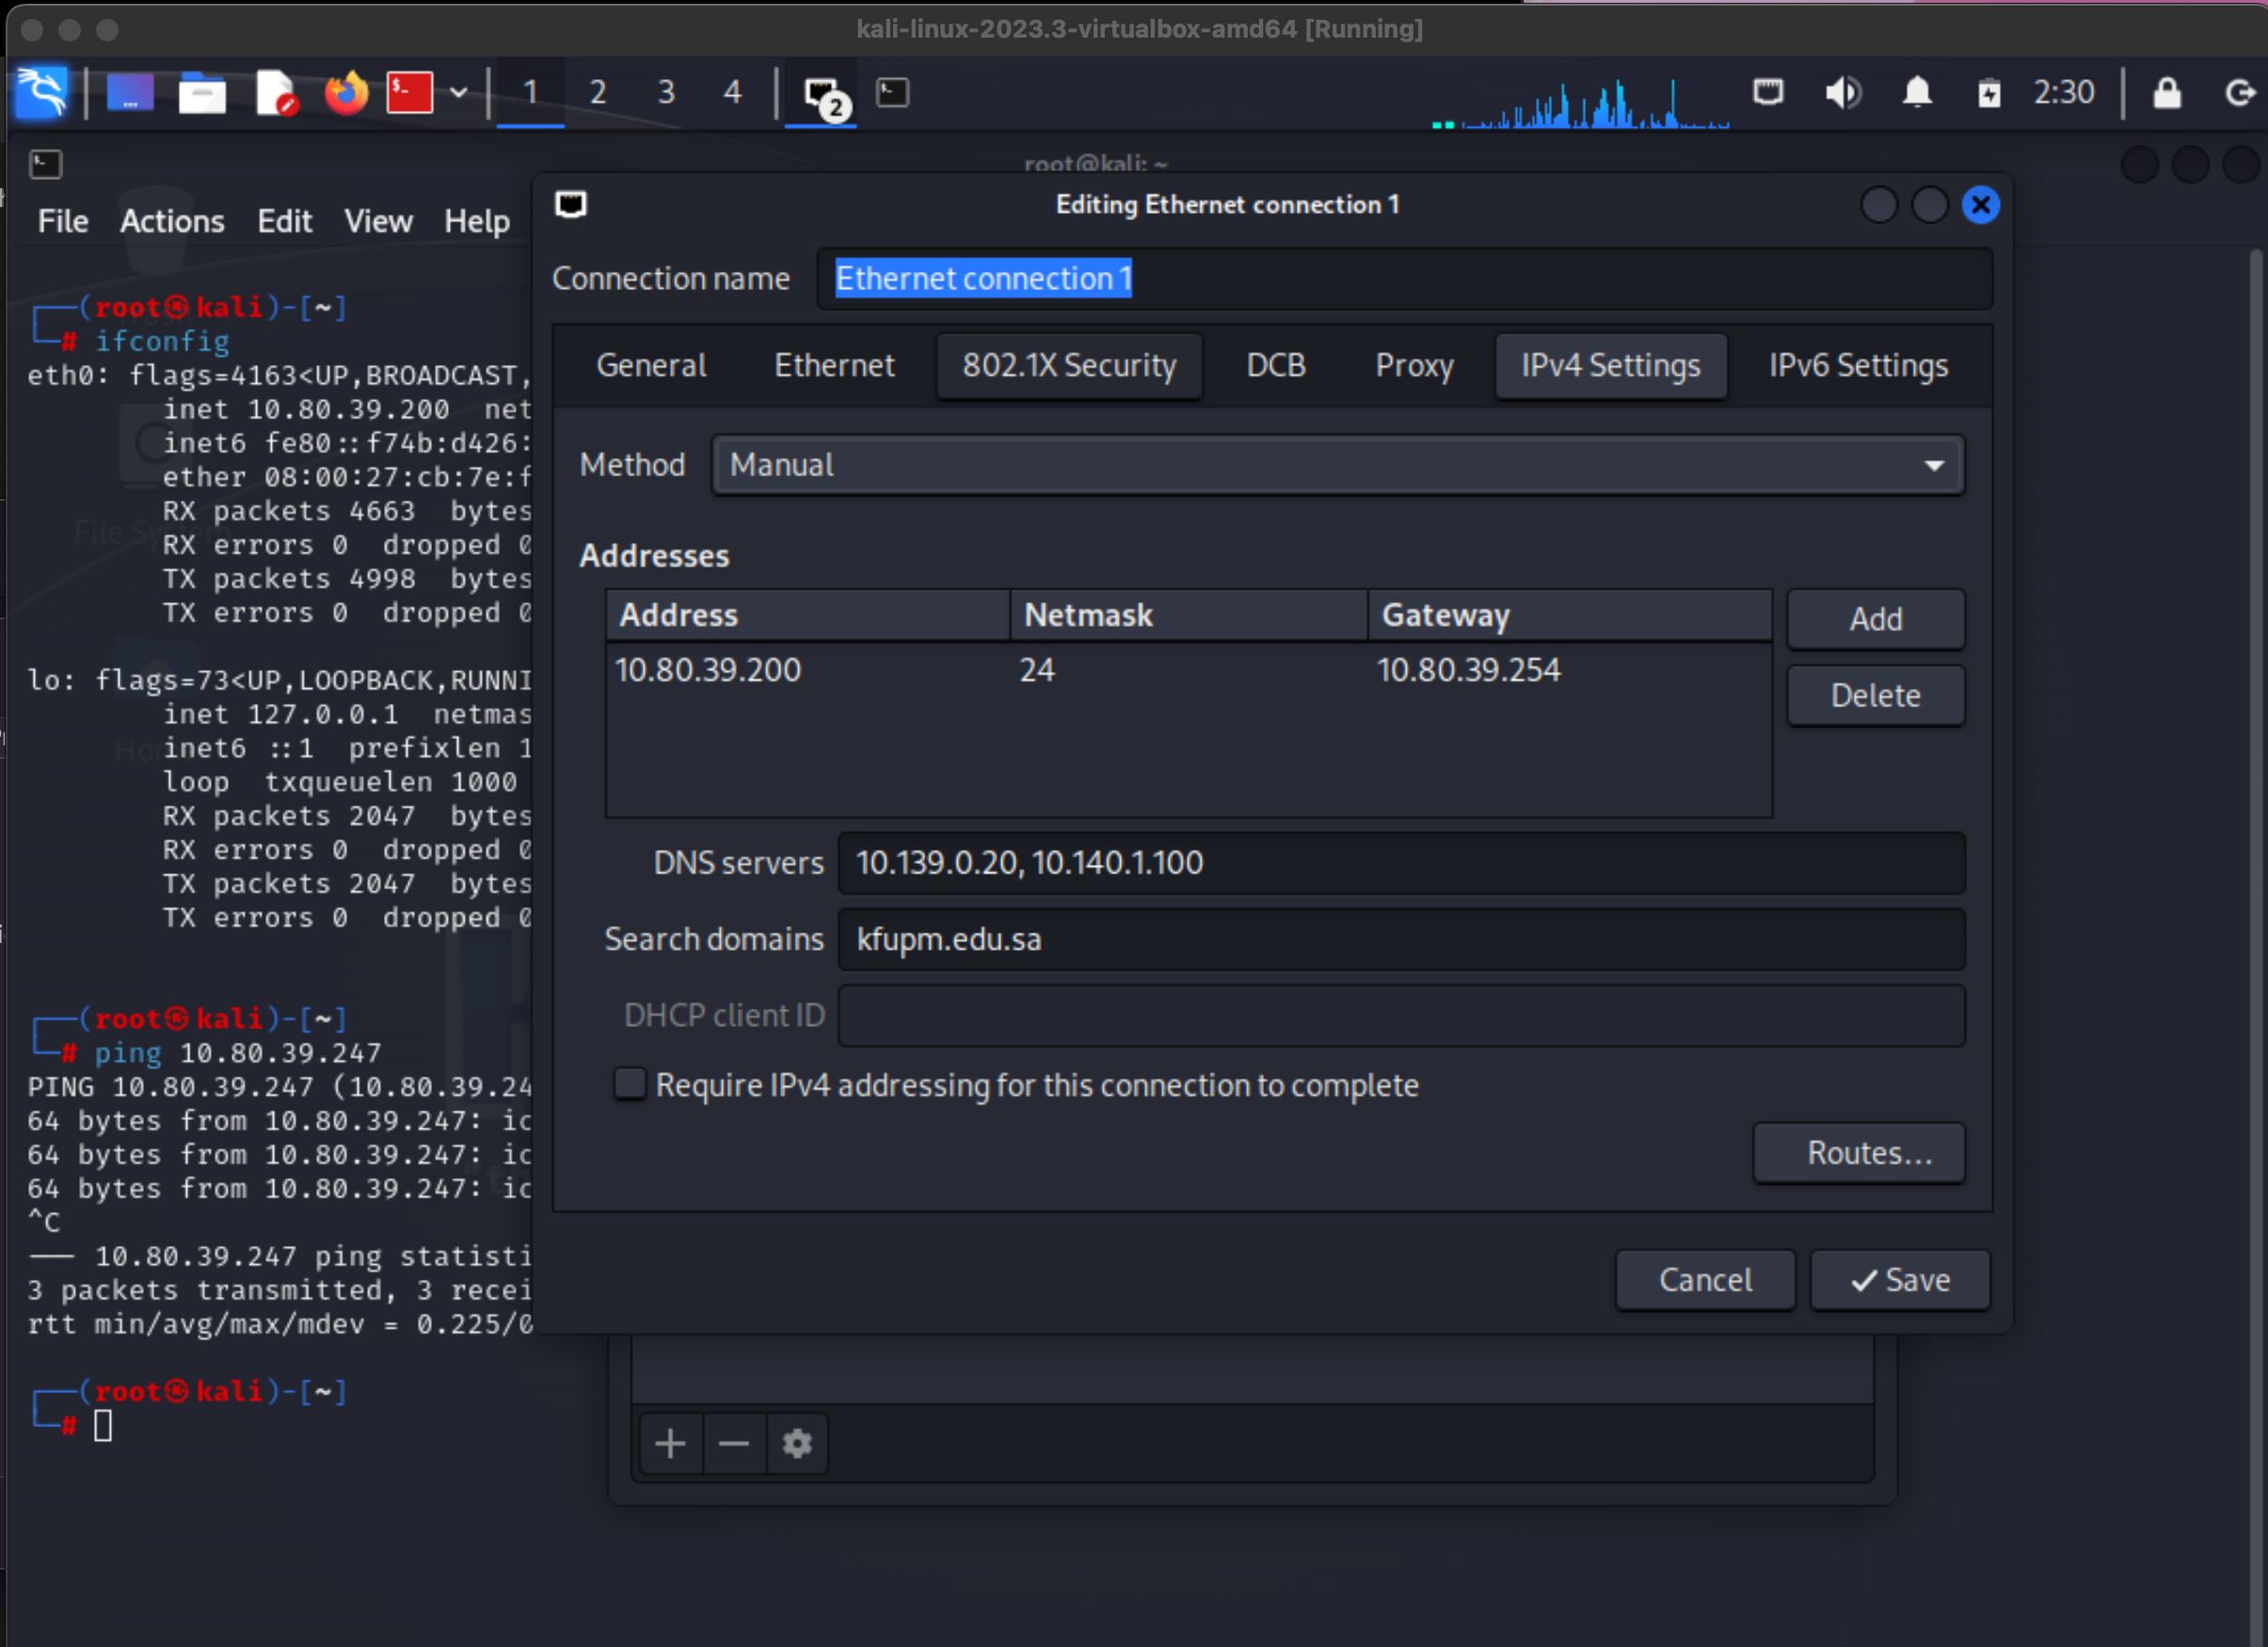
\includegraphics[width=0.95\textwidth]{figures/bridged-set2.png}
	\end{center}
	\caption{For Kali VM I set, IP address to \c{10.80.39.200}, gateway to \c{10.80.39.254}, and the subnet to \c{255.255.255.0} (or 24). And I copied and pasted the same DNS servers as in the hosting OS setting.}
	\label{fig:bridge-kali}
\end{figure}

\begin{figure}
	\begin{center}
		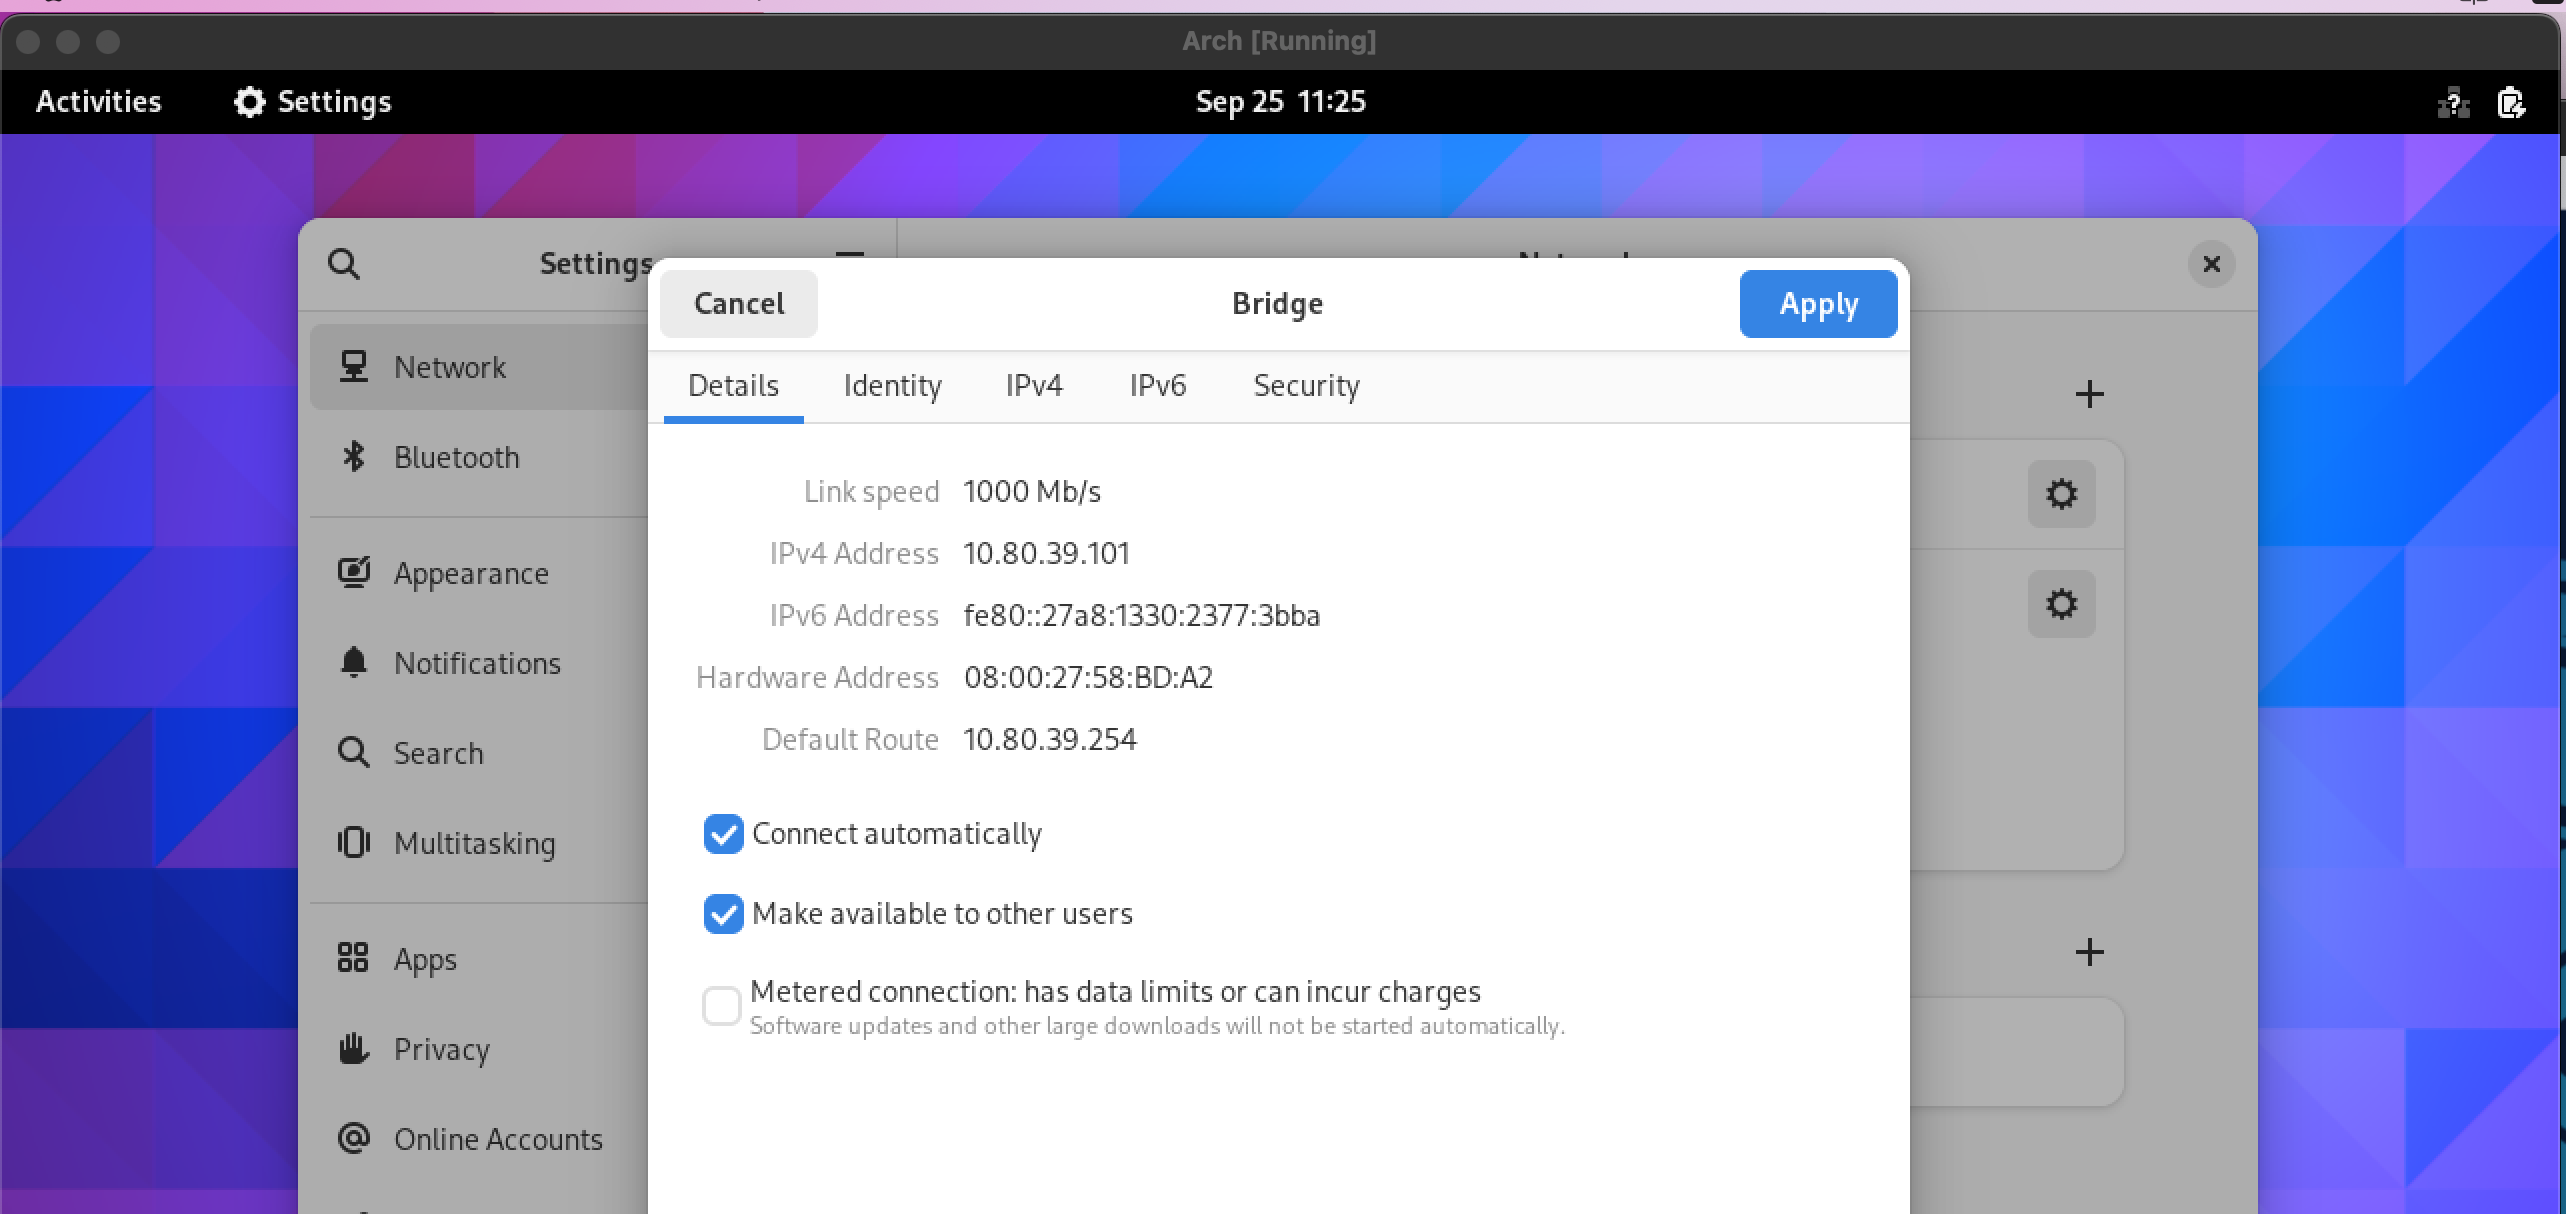
\includegraphics[width=0.95\textwidth]{figures/arch-bridge.png}
	\end{center}
	\caption{Same as in Figure~\ref{fig:bridge-kali} but for Arch VM but IP address is \c{10.80.39.101}}
\end{figure}


\subsection{Host-Only Networking}
Host-Only networking creates a private network that is isolated from both the external network and the host machine's network. VMs with host-only networking can communicate with each other and with the host but cannot access the internet or other external networks directly.


\subsection{Ping each VM}
As in Figure~\ref{fig:ping-vm}, I sent ping request form Kali to Arch, and vice versa. Also I did a ping from my hosting machine
to the both of VM. All ping request had a response ICMP successfully.

\begin{figure}[ht]
	\begin{center}
		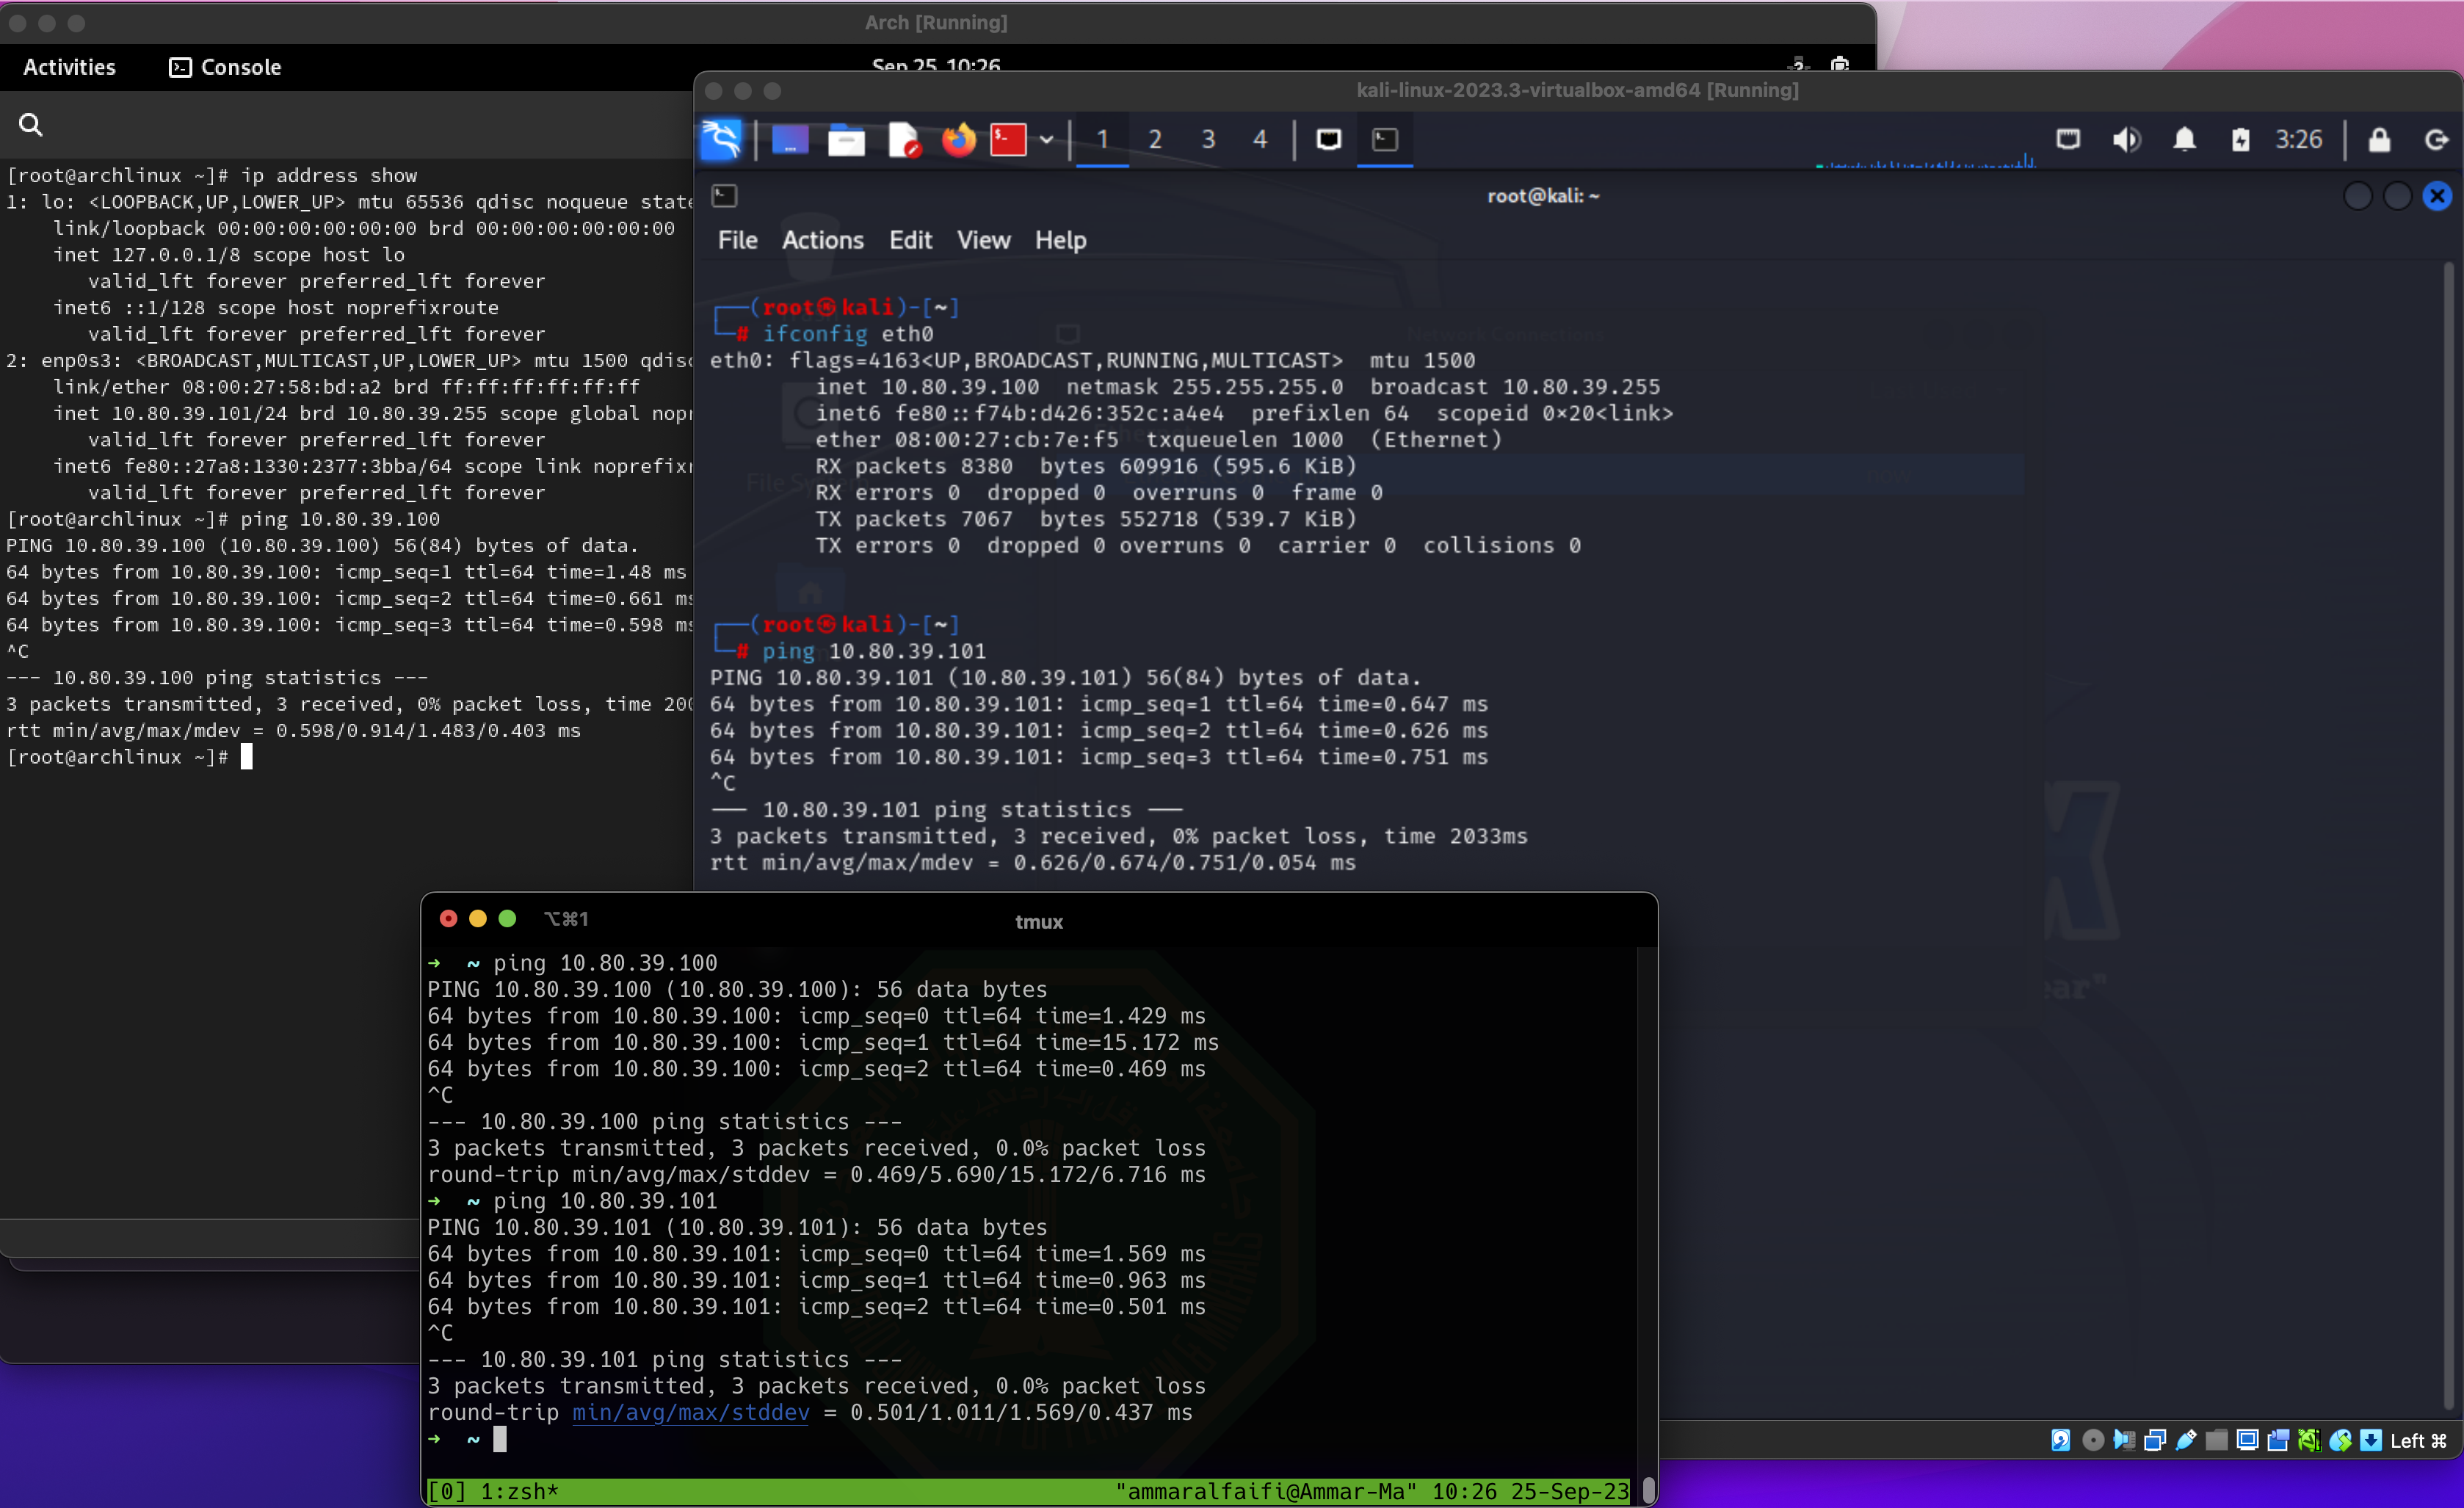
\includegraphics[width=0.95\textwidth]{figures/ping-eachother.png}
	\end{center}
	\caption{Left ping request from Arch to Kali, right is a ping request from Kali to Arch VM, and the middle window is ping request from
		hosting OS to both VMs.}\label{fig:ping-vm}
\end{figure}

\subsection{Accessing Internet} % (fold)
\label{sub:Accessing Internet}
Here I use command \c{curl google.com} to do an HTTPS GET request to the domain \c{google.com}, As in Figure~\ref{fig:access-internet}.

\begin{figure}[ht]
	\begin{center}
		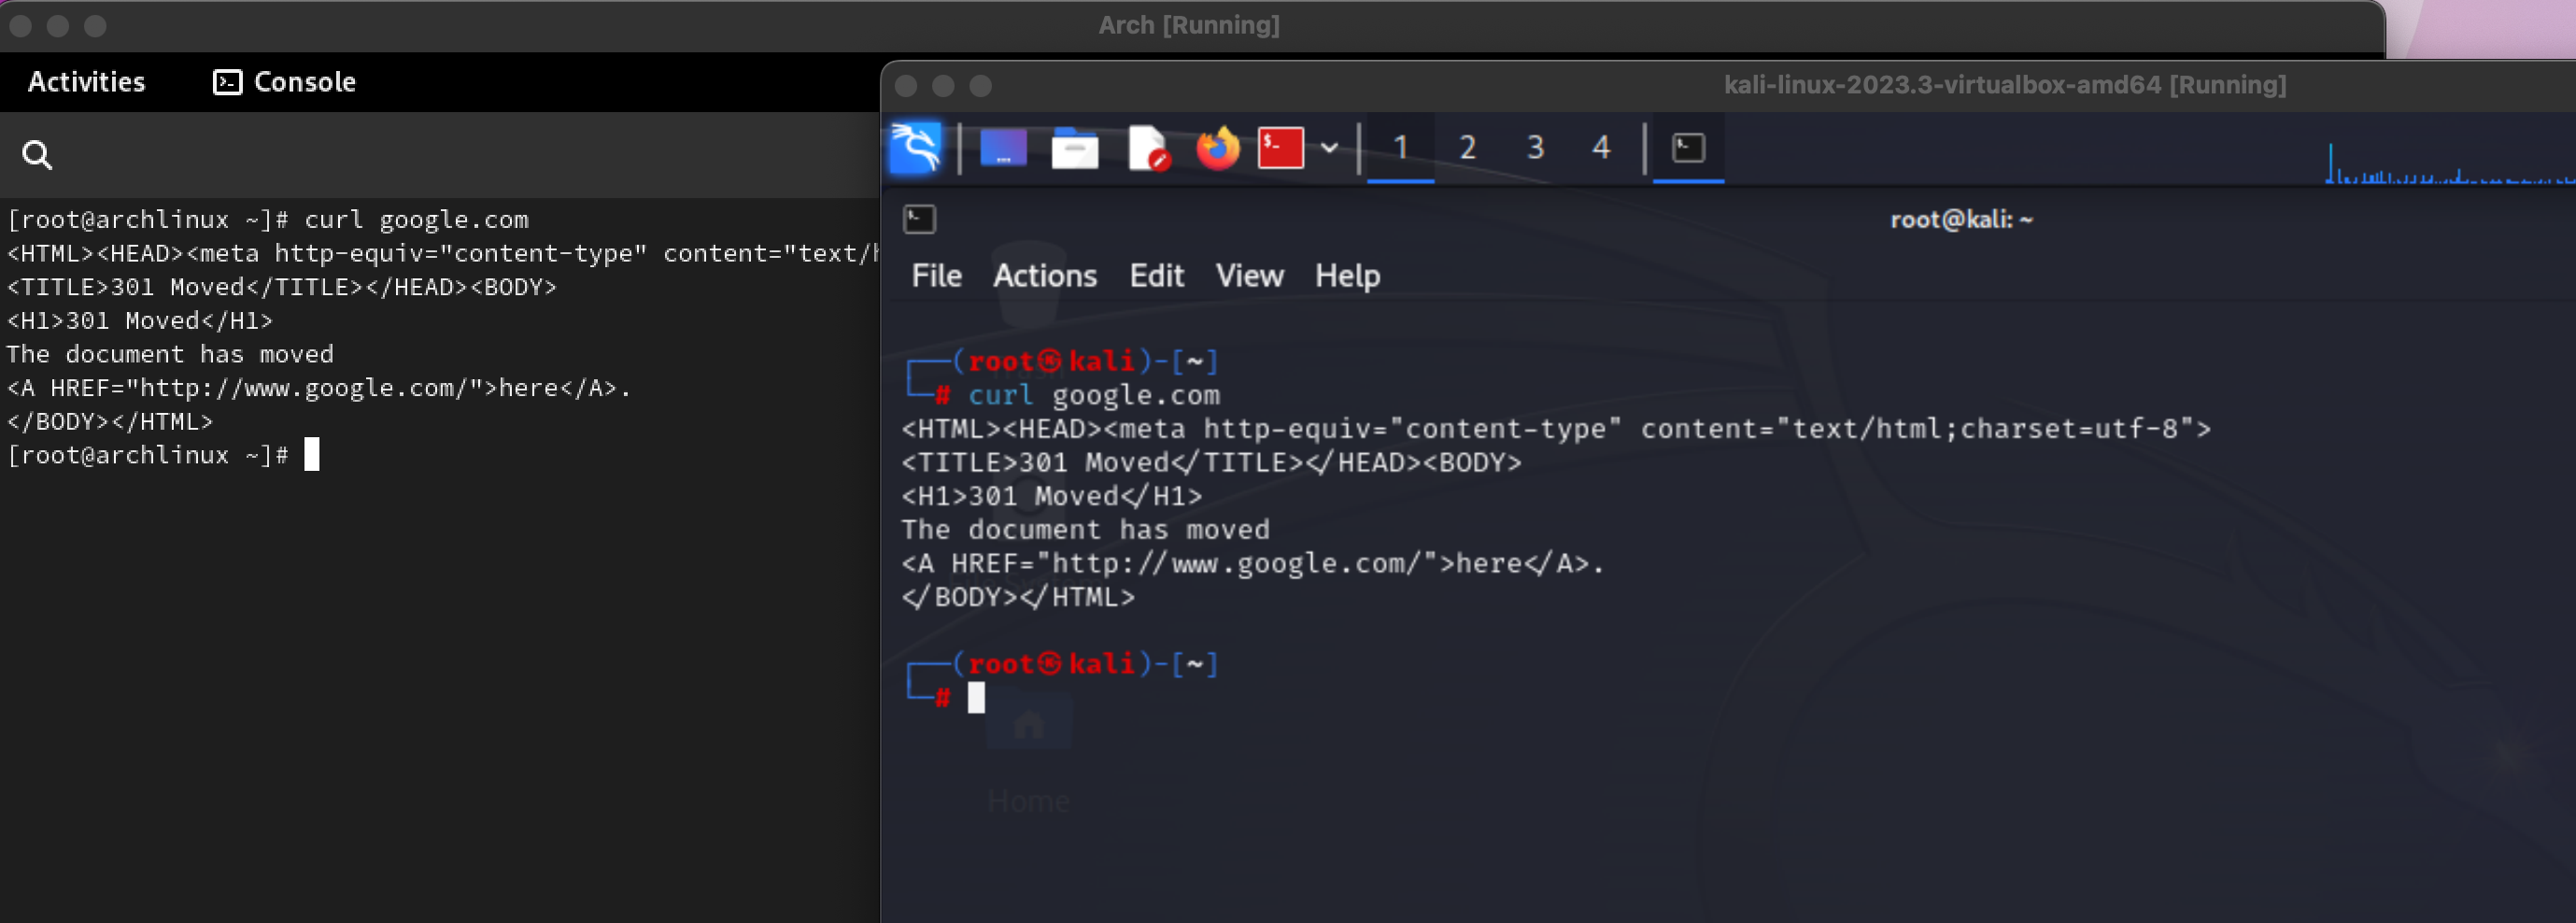
\includegraphics[width=0.95\textwidth]{figures/access-internet.png}
	\end{center}
	\caption{Accessing internet from each VM.}
	\label{fig:access-internet}
\end{figure}


% subsection Accessing Internet (end)


\section{Network Security Tools} % (fold)
\label{sec:Network Security Tools}

\subsection{Using \c{tcpdump}}
TCPdump: Command-line packet analyzer used for capturing and displaying network traffic.

\subsubsection{Filter by IP}
To use \c{tcpdump} and filter by IP address we can use the option \c{host}, which will filter in the any packet carries a source
or destination matching the specifid address, see Figure~\ref{fig:tcpdump-by-ip}

\begin{figure}[ht]
	\begin{center}
		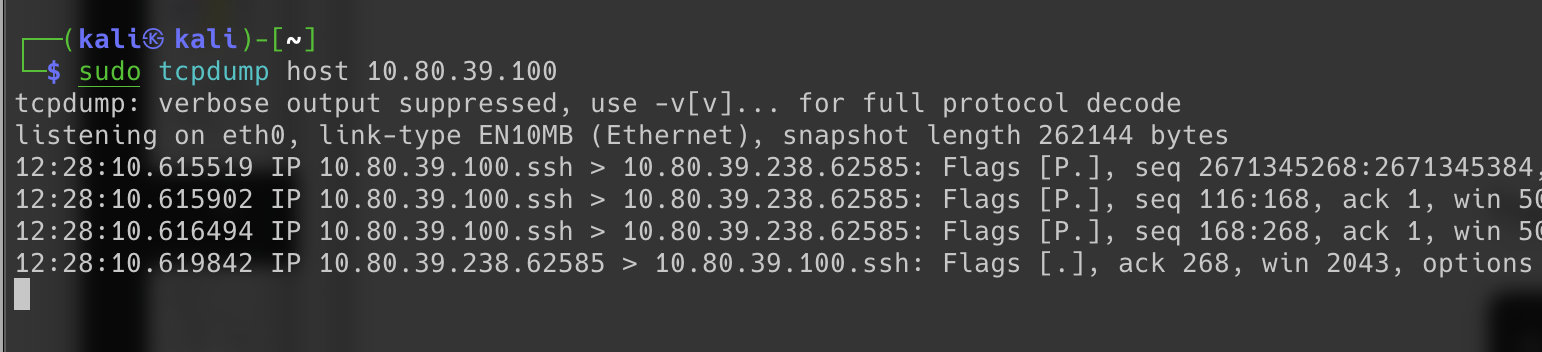
\includegraphics[width=0.95\textwidth]{figures/tcpdump-by-ip.png}
	\end{center}
	\caption{Using tcpdump with filtering by IP addresss, \c{10.80.39.100}, the Kali's IP address.}
	\label{fig:tcpdump-by-ip}
\end{figure}


\subsubsection{Getting password}
I run a simple server on the local host, \c{http://localhost:8000}, which uses unsecure protocol, that is, HTTP (port 8000).
Then I used \c{tcpdump} along with \c{grep} command to filter the packet that contains the `user', as in Figure~\ref{fig:tcpdump-pass}.

\begin{figure}[ht]
	\begin{center}
		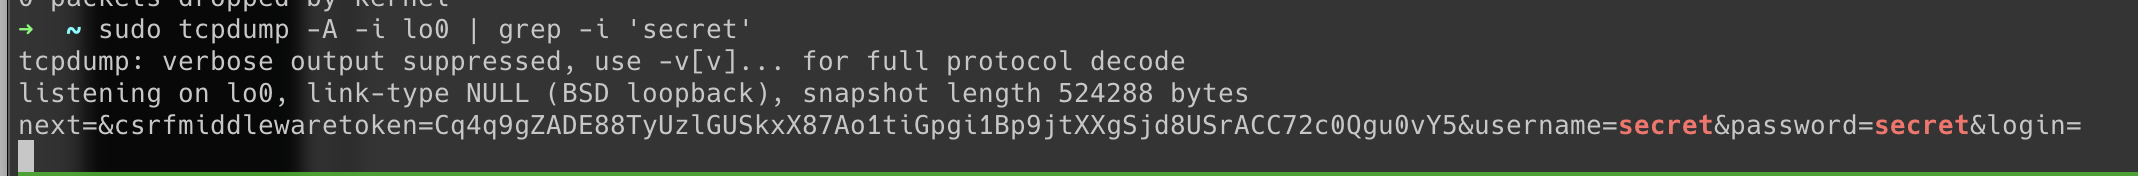
\includegraphics[width=0.95\textwidth]{figures/tcpdump-pass.png}
	\end{center}
	\caption{The username is `secret' and the password is `secret'}
	\label{fig:tcpdump-pass}
\end{figure}


\subsection{Wireshark}
Graphical user interface (GUI) packet analyzer with powerful filtering and analysis capabilities.
Offers a more comprehensive view of captured data with detailed protocol analysis and extensive filtering options.

\subsubsection{Filter by IP}
This is pretty easy in the GUI-based packets analyzer, as Wireshark. See Figure~\ref{fig:wireshark-ip} how I did that.
\begin{figure}
	\begin{center}
		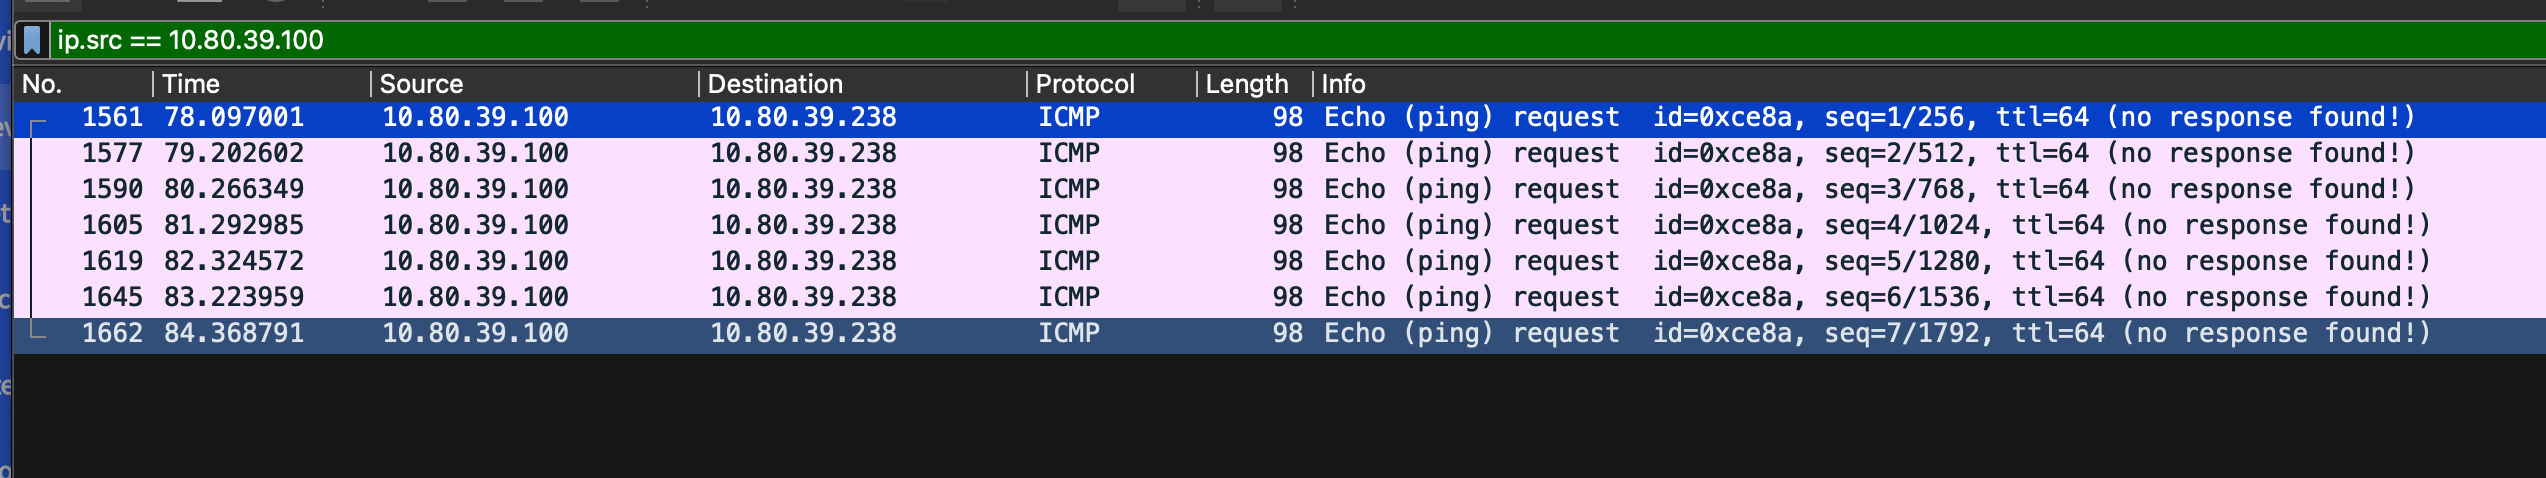
\includegraphics[width=0.95\textwidth]{figures/wireshark-ip.png}
	\end{center}
	\caption{We can filter IP address by writing in this format in the top text area box.}
	\label{fig:wireshark-ip}
\end{figure}

\subsubsection{Getting Password}
It's similar to what I did in Figure~\ref{fig:tcpdump-pass}, but I'll write the filter in the above filters box editing region, as in Figure~\ref{fig:wireshark-pass}.
\begin{figure}
	\begin{center}
		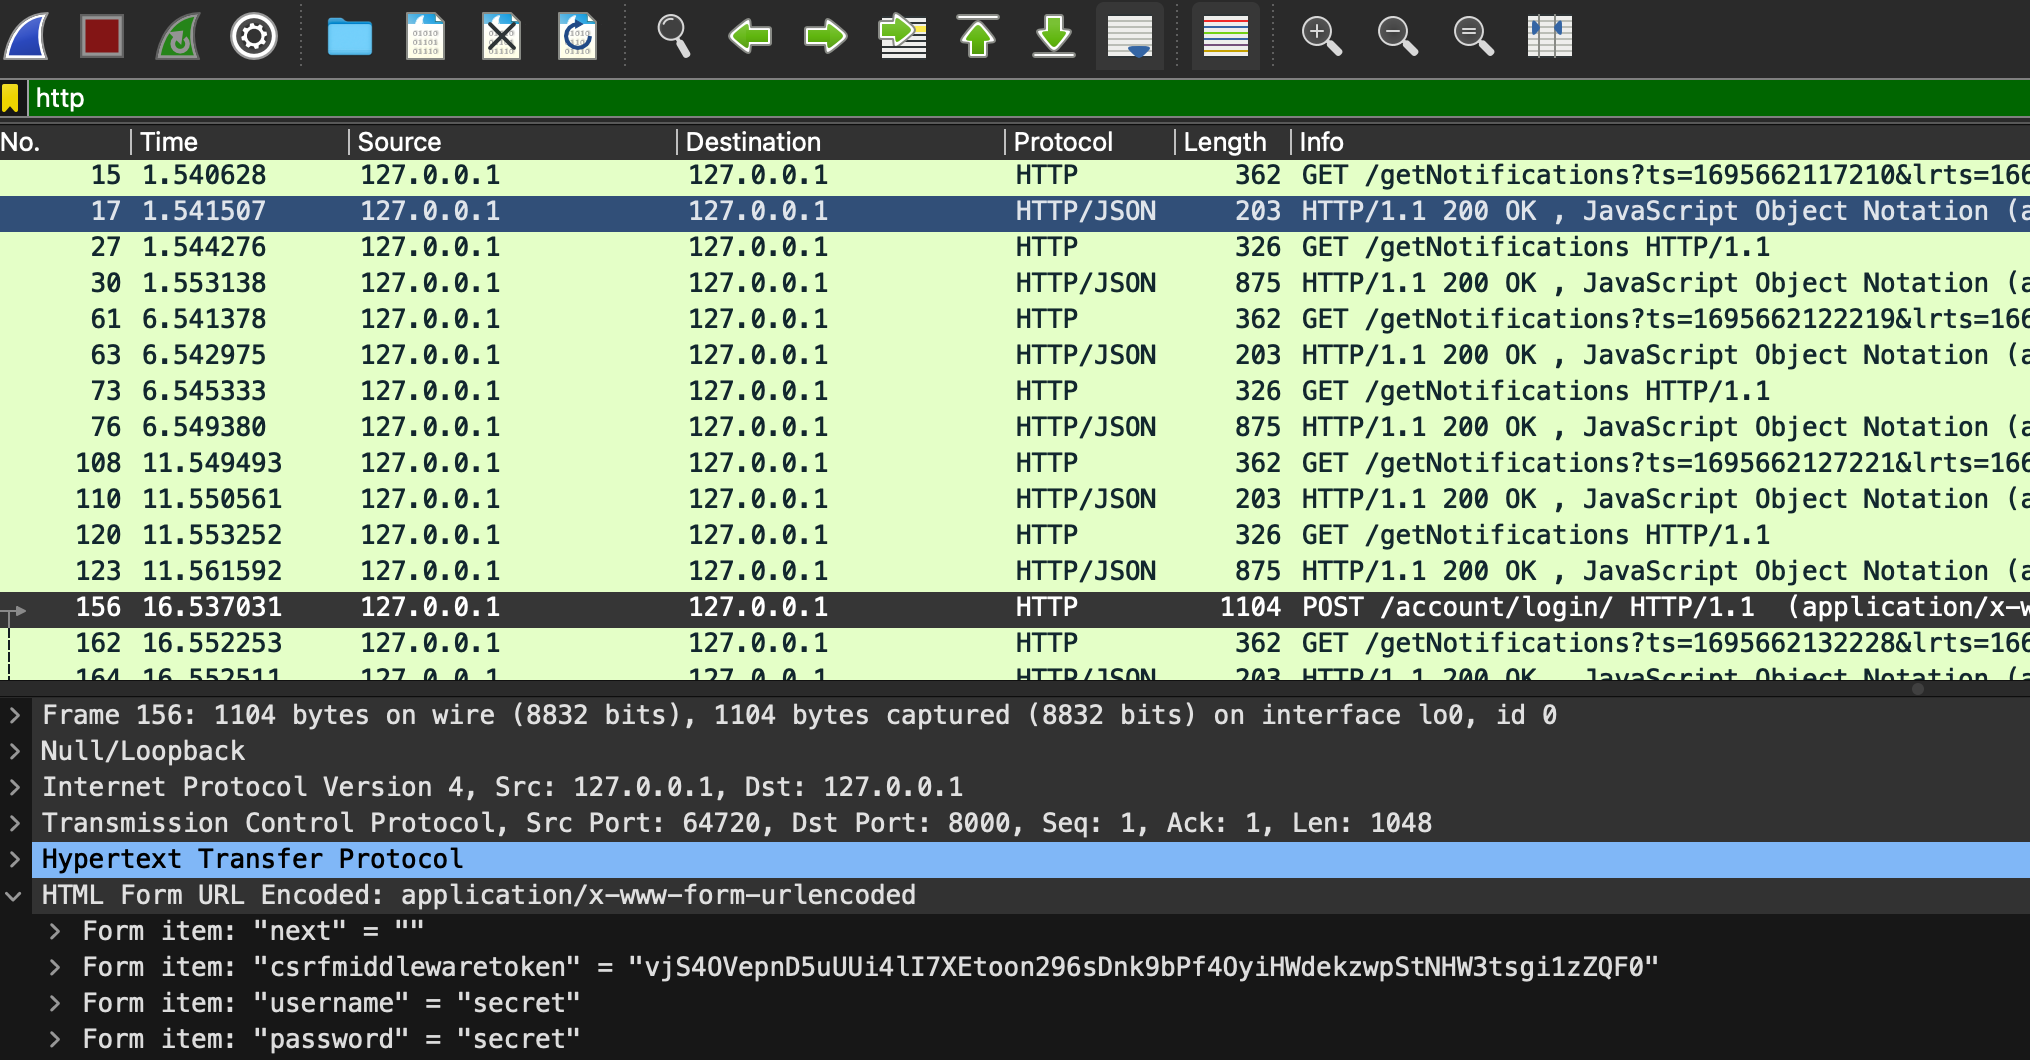
\includegraphics[width=0.95\textwidth]{figures/wireshark-pass.png}
	\end{center}
	\caption{Before launching Wireshark, I chose the Loopvack interface to capture packet from/to my lcoal server. The by using
		http filter I could expose the secret username and password.}
	\label{fig:wireshark-pass}
\end{figure}


\subsection{Using \c{nmap}}
Nmap, short for Network Mapper, is a versatile and widely used network scanning utility known for its multifaceted capabilities. It serves network administrators, security professionals, and penetration testers by providing a comprehensive suite of features, including port scanning, OS detection, service version identification, and extensibility through the Nmap Scripting Engine (NSE).

\subsubsection{Detecting OS of each VM}
Using \c{nmap} along with the option \c{-O}, we can run this command on each IP address of each VM
to detect the OS of each one, see Figure~\ref{fig:nmap-os-detect}

\begin{figure}[ht]
	\begin{center}
		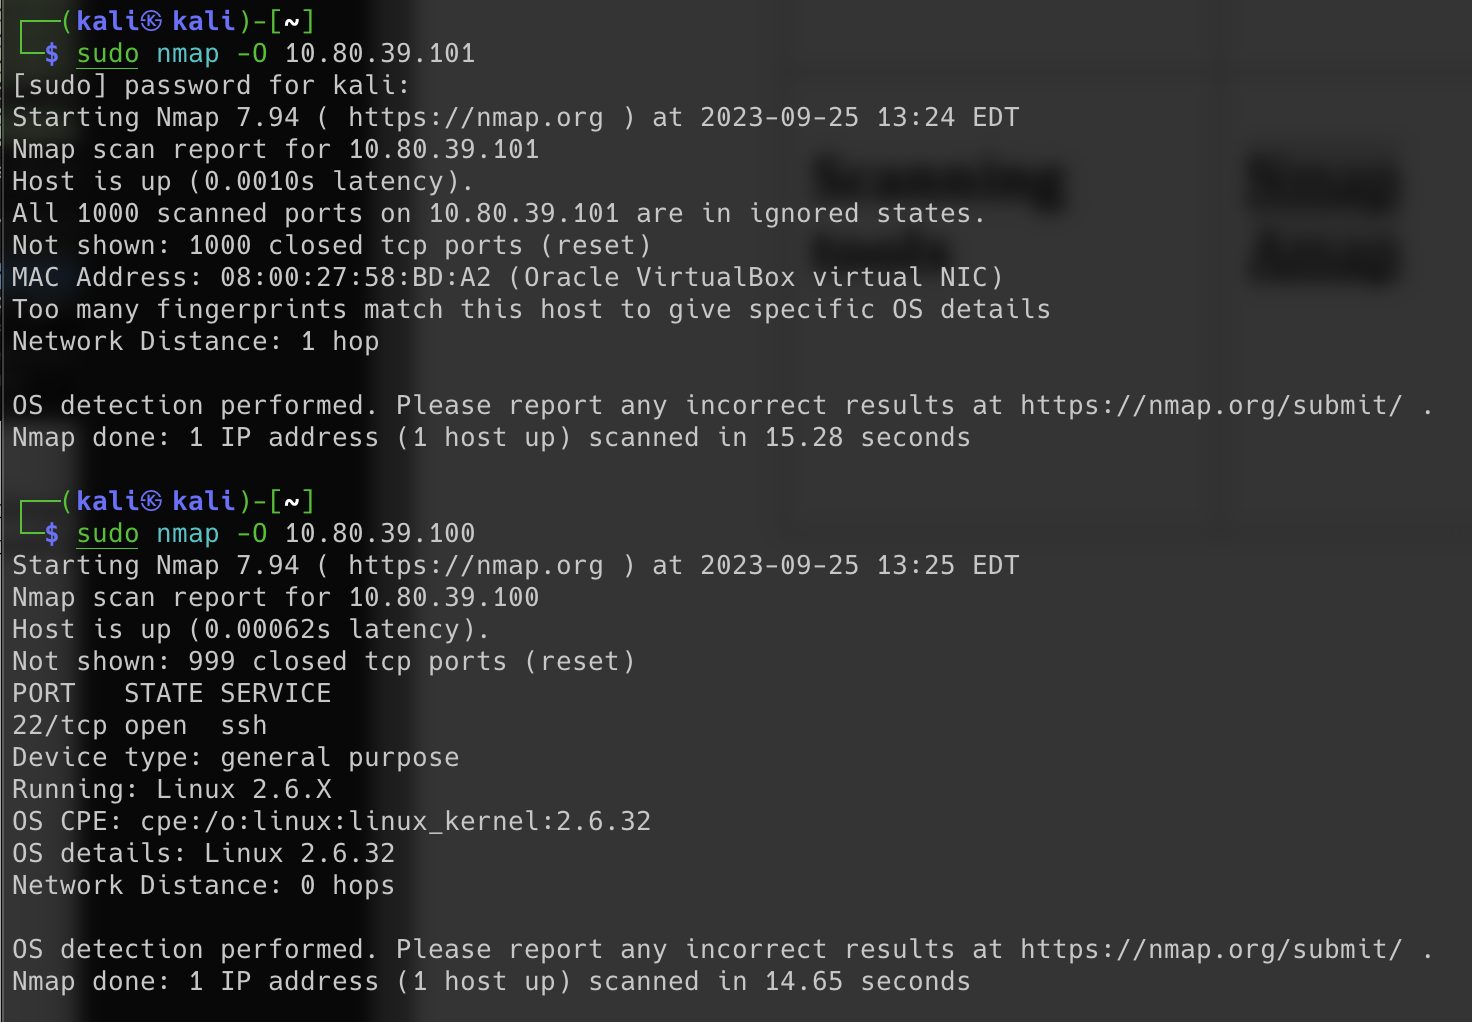
\includegraphics[width=0.75\textwidth]{figures/nmap-os-detect.png}
	\end{center}
	\caption{First run is to detect OS of Arch VM, the second run is to detect OS of the Kali VM.}
	\label{fig:nmap-os-detect}
\end{figure}

\subsubsection{Scan All Reserved Ports}
To use \c{nmap} to scan all reserved ports we run the command \c{nmap -p 0-1023 IP\_ADDRESS}, as I did in Figure~\ref{fig:nmap-scan}

\begin{figure}[ht]
	\begin{center}
		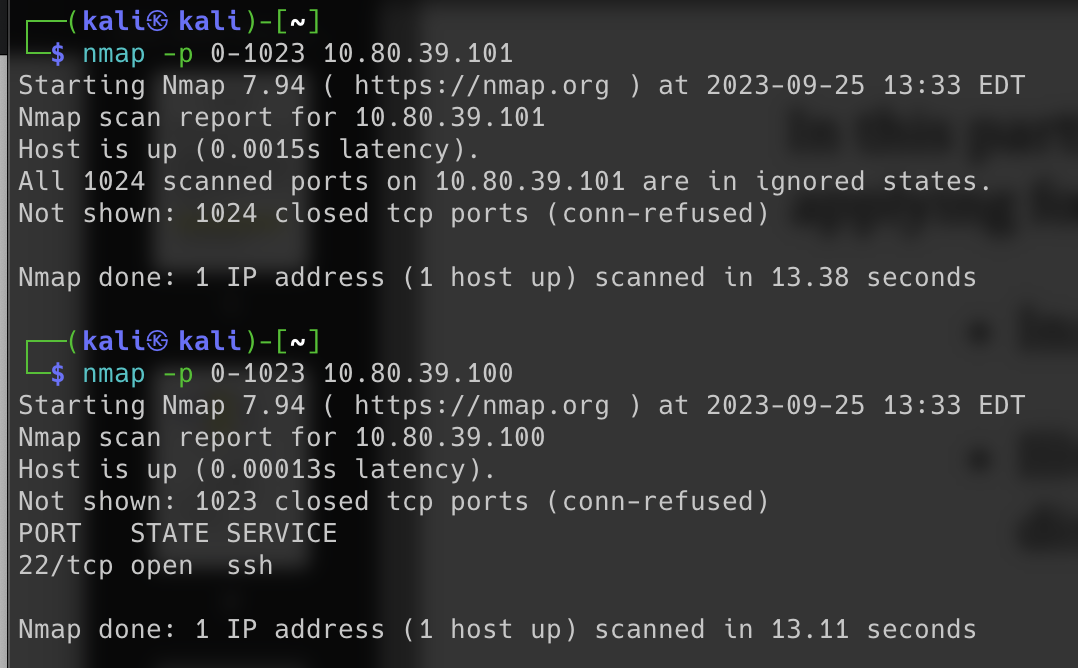
\includegraphics[width=0.75\textwidth]{figures/nmap-scan.png}
	\end{center}
	\caption{First run is to scan all reserved ports on Arch VM and the second run is for Kali VM. Note for Kali I run a \c{ssh} server to ease connecting to it, that's why it shows port 22 is awake.}\label{fig:nmap-scan}
\end{figure}


\subsection{Using \c{amap}}
Amap, or Application Mapper, focuses on a specialized niche within network scanning. Its primary mission is the precise identification of network services and applications running on open ports. Amap excels at this task by employing targeted probes and scrutinizing responses, making it especially adept at pinpointing less common or obscure services.

\subsubsection{Detecting OS of each VM}
\c{amap} is outdated, I could not find a binary for it nor it was bundled with Kali. I tried to build it form source but it requires old legacy libs so I gave up.


\end{document}
